\documentclass{beamer}
\usetheme{Copenhagen}

%\setbeamercolor{frametitle}{fg=white}
%\setbeamercolor{background canvas}{bg=black}
%\setbeamercolor{normal text}{fg=white}

% Title page details:
\title{Genetic signatures of evolutionary rescue}
\author{Matthew Osmond}
\institute{Department of Ecology and Evolutionary Biology\\ University of Toronto}
\date{\today}

\begin{document}

% ==============================================

\begin{frame}
	\titlepage
\end{frame}

% ==============================================

% at least 27 yrs of theory on evol rescue: we know a lot about when and how rescue should occur
% a large and quickly growing number of experiments of increasing complexity and detail: verifying theory and discovering additional factors
% many examples of drug resistance, eg HIV, in asexual microbes: stressing an applied need to understand rescue for human health
% a big question that remains is: how common is rescue in wild sexual species? conservation angle
% evidence of the excitement around this question: a recent spike in claims for rescue in wild sexual species (amaranthus, killifish, arabidopsis, bats, etc)
% however, still unclear how confidently we can identify rescue from (predominately) contemporary genetic data
% this is a new direction for rescue theory

% ==============================================

\begin{frame}
	\frametitle{Evolutionary rescue}

	\begin{center}
		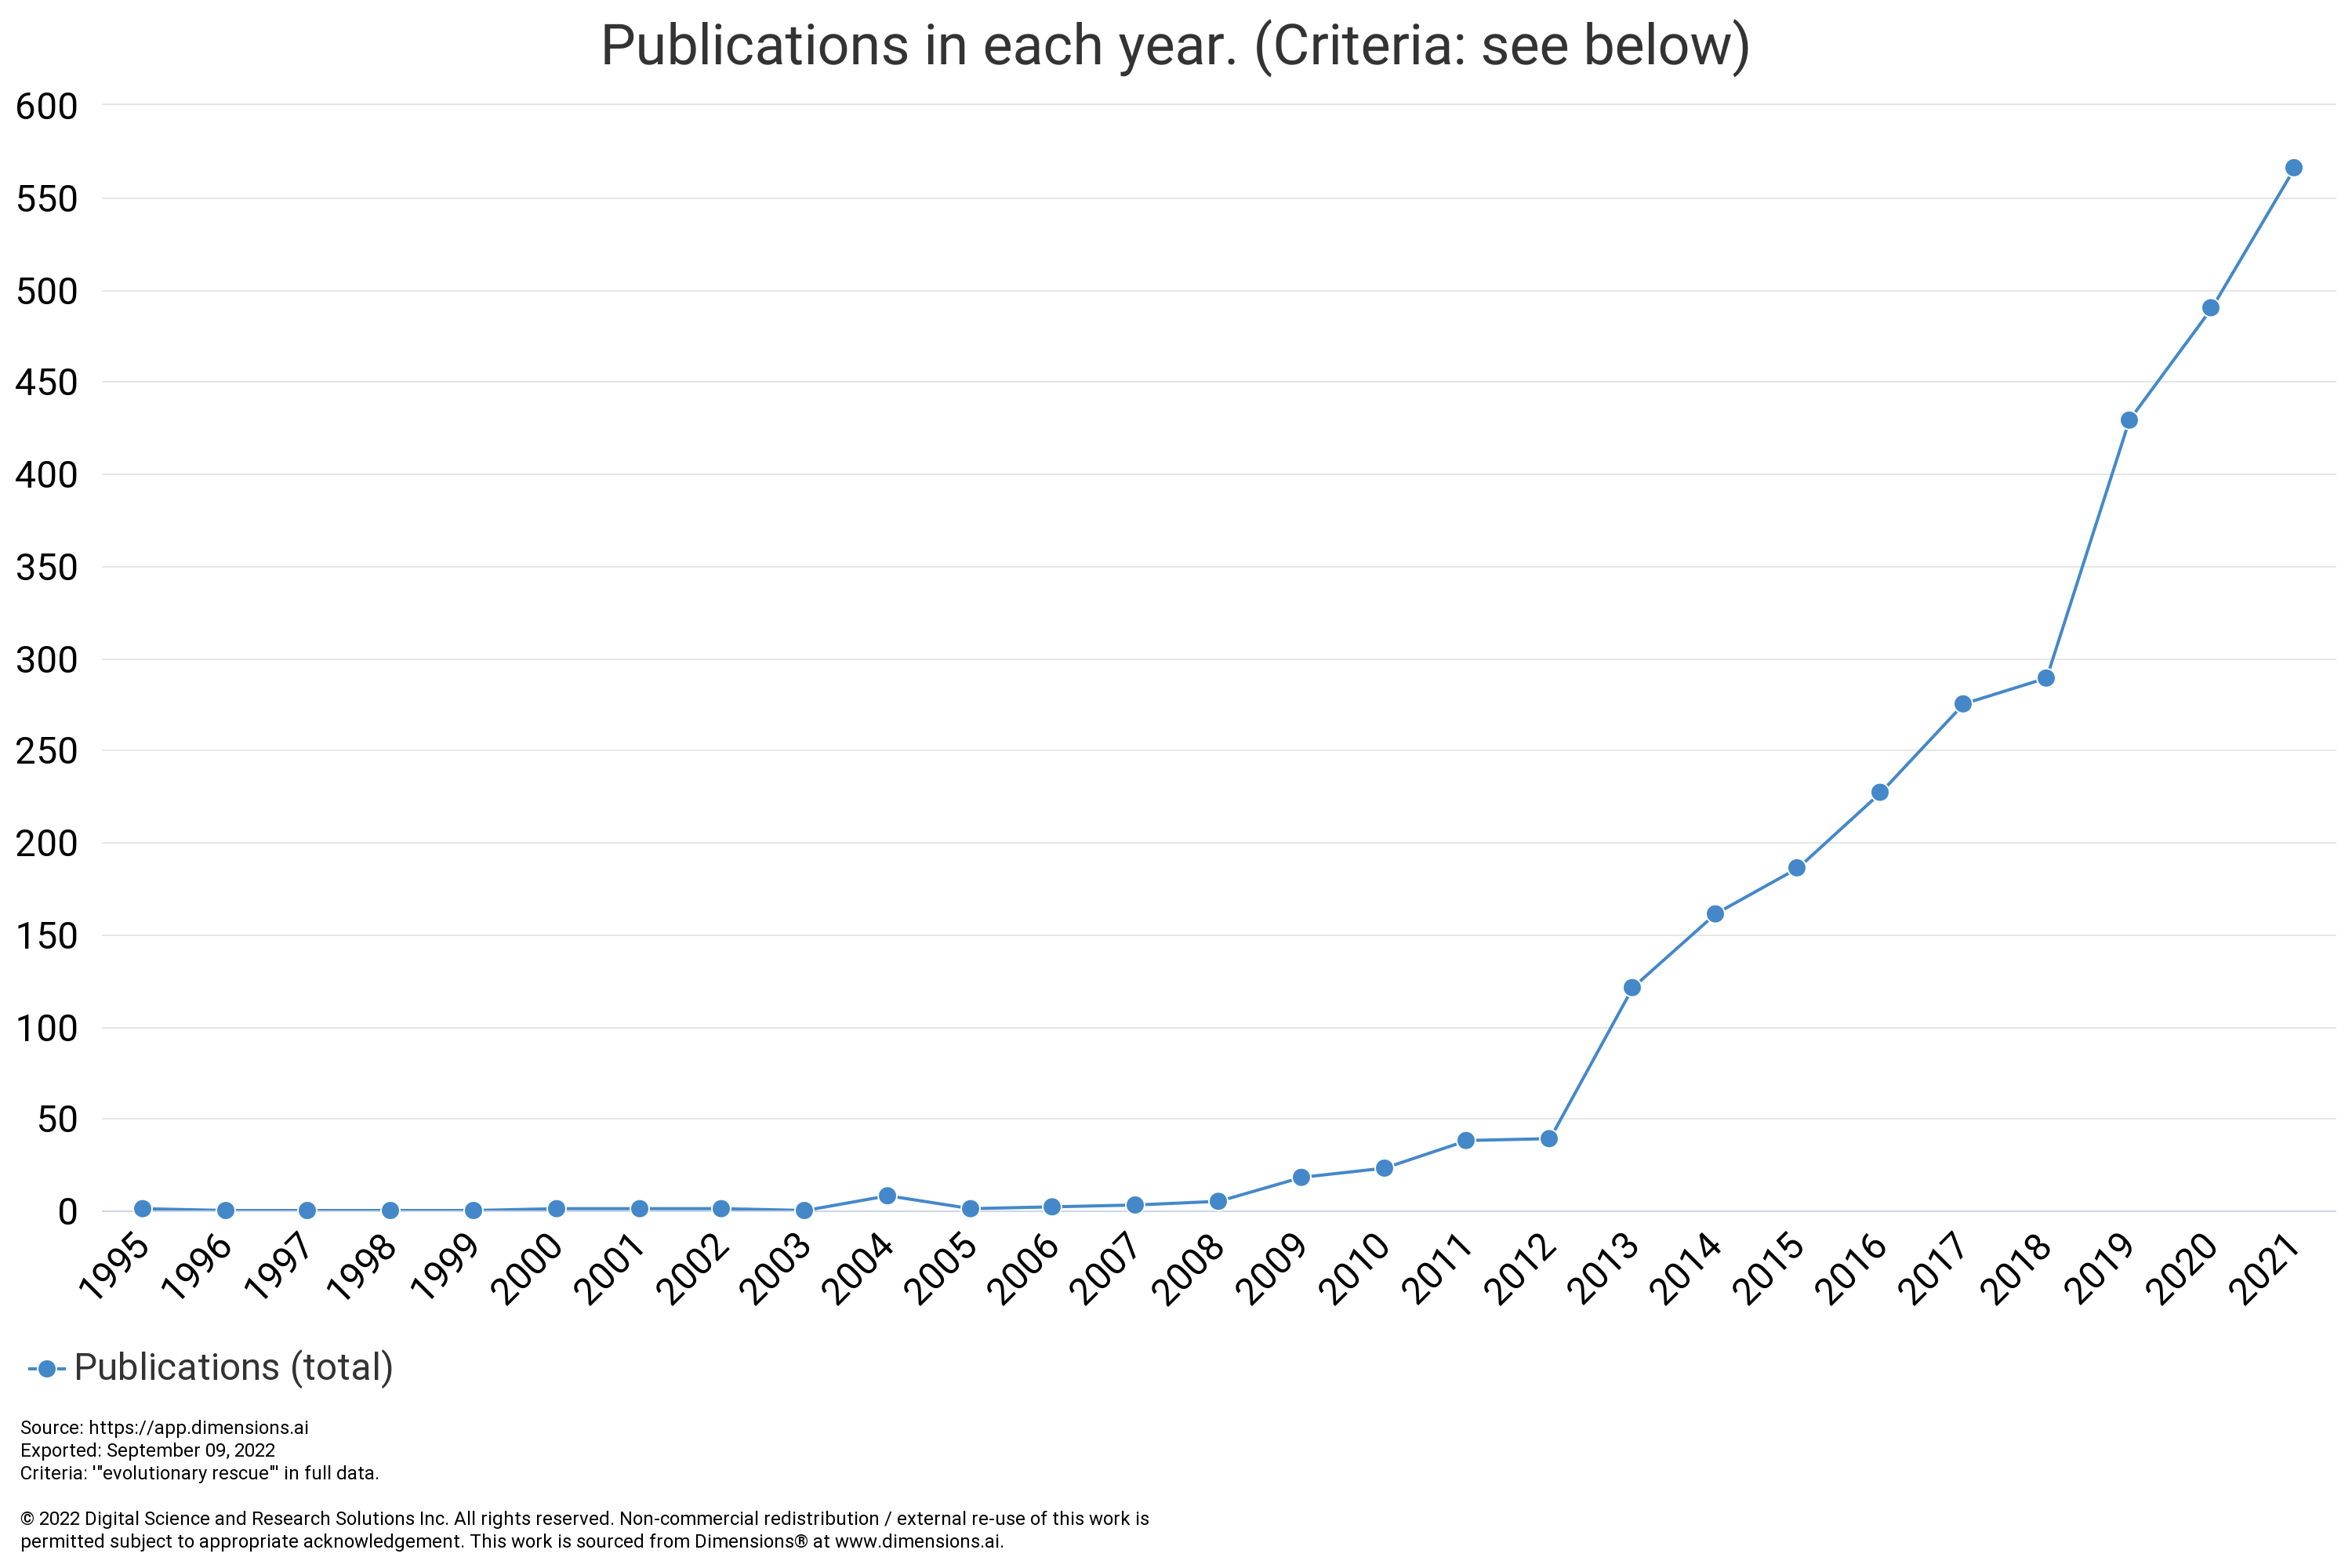
\includegraphics[width=\linewidth]{../images/er-trend.png}
	\end{center}

\end{frame}

% ==============================================

\begin{frame}
	\frametitle{State of the field}

	\begin{itemize}
		\item we have a lot of theory on when/how rescue should happen \pause
		\item we have a lot of examples of rescue in asexual microbes \pause
		\begin{itemize}
			\item important for drug resistance \pause
		\end{itemize}
		\item a big question remains \pause
	\end{itemize}

	\begin{block}{Q}
		How common is rescue in wild sexual species?
	\end{block}

	\begin{itemize}
		\item important for conservation
	\end{itemize}

\end{frame}

% ==============================================

\begin{frame}
	\frametitle{How common is rescue in wild sexual species?}

	\begin{alertblock}{To do}
		images of organisms
	\end{alertblock}

	A lot of excitement around this question right now, eg \pause

	\begin{itemize}
		\item Hares rescued from lack of snow (Mills et al. 2018) \pause
		\item Bats rescued from white-nose syndrome (Gignoux-Wolfsohn et al. 2018) \pause
		\item Killifish rescued from pollution (Oziolor et al. 2019) \pause
		\item \textit{Amaranthus tuberculatus} rescued from herbicides (Kreiner et al. 2019) \pause
		\item \textit{Arabidopsis thaliana} rescued from dry new climate (Fulgione et al. 2022)
	\end{itemize}

\end{frame}

% ==============================================

\begin{frame}
	\frametitle{How common is rescue in wild sexual species?}

	\begin{itemize}
		\item for most wild species all we have is contemporary data \pause
	\end{itemize}

	\begin{block}{Q}
		Can we infer past rescue from a bunch of genomes?
	\end{block}

\end{frame}

% ==============================================

% coalescent framework for detecting selection and demography
% work with Coop on signatures of rescue: difficult/impossible to differentiate sweep+bottleneck from any data, but especially summary statistics?

% ==============================================


\begin{frame}
	\frametitle{Can we infer past rescue from a bunch of genomes?}

	\begin{alertblock}{To do}
		plot from our paper
	\end{alertblock}

	\begin{itemize}
		\item Graham Coop and I started down this path (Osmond \& Coop 2020) \pause
		\item coalescent model of rescue via a selective sweep \pause
		\item concluded that it is very difficult to infer rescue from summary statistics \pause
	\end{itemize}

	\begin{block}{Q}
		But what if we could observe the coalescent itself?
	\end{block}

\end{frame}

% ==============================================

% what if we could see the coalecent trees themselves? does that give us more power to detect rescue? (Hejase et al 2022 say that summary statistics confound seln and demo)
% arabidopsis example (https://www.nature.com/articles/s41467-022-28800-z): used the trees, found bottleneck and sweeps but remains unclear how well their methodology can pick up rescue

% ==============================================

\begin{frame}
	\frametitle{But what if we could observe the coalescent itself?}

	\begin{alertblock}{To do}
		plot of trees
	\end{alertblock}

	\begin{itemize}
		\item recent advances allow us to infer the coalescent trees \pause
		\begin{itemize}
			\item ARGweaver (Rasmussen \& Siepel 2013) \pause
			\item Relate (Speidel et al. 2019) \pause
		\end{itemize}
	\end{itemize}

\end{frame}

% ==============================================

\begin{frame}
	\frametitle{But what if we could observe the coalescent itself?}

	\begin{alertblock}{To do}
		plot of demo and evol inference
	\end{alertblock}

	\begin{itemize}
		\item these trees have a lot of power to infer recent demography and evolution \pause
		\begin{itemize}
			\item show relate demography inference plot
			\item CLUES (Stern et al. 2019) \pause
		\end{itemize}
	\end{itemize}

\end{frame}

% ==============================================

\begin{frame}
	\frametitle{But what if we could observe the coalescent itself?}

	\begin{alertblock}{To do}
		plots from papers
	\end{alertblock}

	\begin{itemize}
		\item already been used for rescue, eg \pause
		\begin{itemize}
			\item Kreiner et al. 2022 (ARGweaver, Relate) \pause
			\item Fulgione et al. 2022 (Relate, CLUES) \pause
		\end{itemize}
	\end{itemize}

	\begin{block}{Q}
		How well do inferred trees infer rescue?
	\end{block}

\end{frame}

% ==============================================

% run simulations of rescue, infer trees, infer demography and selection -- can we detect rescue?

% ==============================================

\begin{frame}
	\frametitle{How well do inferred trees infer rescue?}

	\begin{itemize}
		\item simulate rescue via selective sweep in SLiM (Haller et al. 2019) \pause
		\item infer trees from resulting VCF \pause
		\item infer demography and allele frequency dynamics from trees \pause
		\item compare with the truth
	\end{itemize}

\end{frame}

% ==============================================

\begin{frame}
	\frametitle{How well do inferred trees infer rescue?}

	\begin{itemize}
		\item control: inferring a sweep with constant population size \pause
	\end{itemize}

	\begin{center}
		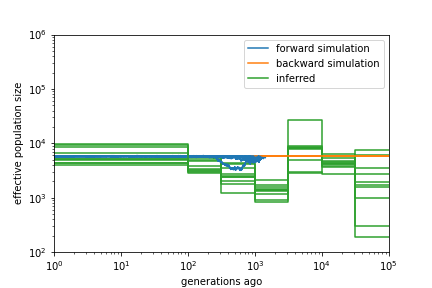
\includegraphics[width=0.5\linewidth]{{../images/sim_10000K_0d_0.01s_0.5h_2B_0u_1q_1000000L_1.25e-08r_0.75f_10n_25k_2.5e-08U}.png}
	\end{center}

\end{frame}

% ==============================================

\begin{frame}
	\frametitle{Conclusion}

\end{frame}

% ==============================================


% speidel et al 2019 show that they can infer demography better than SMC in recent time, 10^2 - 10^4 generations (fig 2)
% stern et al 2019 show that they can infer allele freq and selection very well, including recent strong selection (<10^2 gens, s<0.03) from SGV or DNM (fig 7a)
% stern et al 2019 used ARGweaver but later updated the software to work with Relate, which is what Fulgione used
% hejase et al 2022: relate and SIA better at detecting seln than sum stats when selection weak and DAF low (fig 2); CLUES tends to understimate strong seln coefficients with true trees (fig 3), CLUES very much underestimates s when using inferred Relate trees (fig 4) -- note that comparing this to stern et al 2019 means that the error is coming from Relate, and that ARGweaver should do better, compare fig 4 and s5 in hejase (clues better with argweaver, but still not great and a TON of variation)

\end{document}
